\documentclass[12pt]{exam}
\usepackage{amsmath}
\usepackage{amssymb}
\usepackage{amsthm}
\usepackage{tikz}
\usepackage{mathtools}
\usepackage{graphicx}
\usepackage{wrapfig}

\usepackage{bm} %bold symbols
\usepackage{hyperref} %add links

%%%%%%%%%%%%%%%%%%%%%%%%%
% 	Define vars here 	%
%%%%%%%%%%%%%%%%%%%%%%%%%

\def\hwName{Homework Set 3: §13.1 - 13.4}
\author{Zhengyu James Pan} %use like \@author
\def\email{jzpan@umich.edu}
\makeatletter

\begin{document}
%Header
\pagestyle{head}
\firstpageheader{}{}{}
\header{MATH 215}{\hwName}{\thepage}

%Solution formatting
\printanswers
\unframedsolutions

%Top matter
{\parindent0in
\begin{center}
	\bf MATH 215 FALL 2023\\
	\bf \hwName \\
	\@author\ (\href{mailto:\email}{\email})
\end{center}
}

\begin{questions}
%1
\question Do exercises 25-30 of §13.1 of \textit{Stewart’s Multivariable Calculus}.
	\\\\\textbf{Solutions:}
	\begin{questions}
		\setcounter{question}{24}
		\question \boxed{II} -- since $\sin(t)$ and $]cos(t)$ are multiplied by $t$, there is a spiral as circular arcs with increasing radius. y increases linearly.
		\question \boxed{VI} -- circles with a sudden jump in z, corresponding to the asymptote in $\frac{1}{1+t^2}$
		\question \boxed{V} -- 
		\question \boxed{I} 
		\question \boxed{IV}
		\question \boxed{III}
	\end{questions}
\clearpage
\setcounter{question}{1}
%2
\question Show that the space curve with parametric equation $\mathbf{r}(t) = \langle t^2 - 1, 6 + 3t - t^2, 4 - 6t\rangle$ lies in a plane, and find the equation of this plane. \textit{Hint}: If $r(t)$ lies in a plane, what must be true for $\mathbf{r'}(t)$?
	\begin{solution}
		We find the tangent vector to this curve, allowing us to search for possible normal vectors.
		\[ \mathbf{r'}(t) = \langle 2t, 3 - 2t, -6 \rangle\]
		We can see that the vector $\langle 2, 2, 1 \rangle$ will always be orthogonal with this curve, as dotting it with the tangent vector always grants 0. Thus, it lies in a plane with equation
		\[ \boxed{2(x + 1) + 2(y - 6) + (z - 4) = 0}. \tag*{\qed} \]
	\end{solution}
\clearpage

%3
\question 
	\begin{parts}
		\part Draw and parametrize the circle of radius 2 centered at $(1, 2, 0)$ and lying on the plane $x + y + z = 3$. It may help to find two orthogonal unit vectors parallel to the plane.
		\begin{solution}

			
			

			\tikzset{every picture/.style={line width=0.75pt}} %set default line width to 0.75pt        

			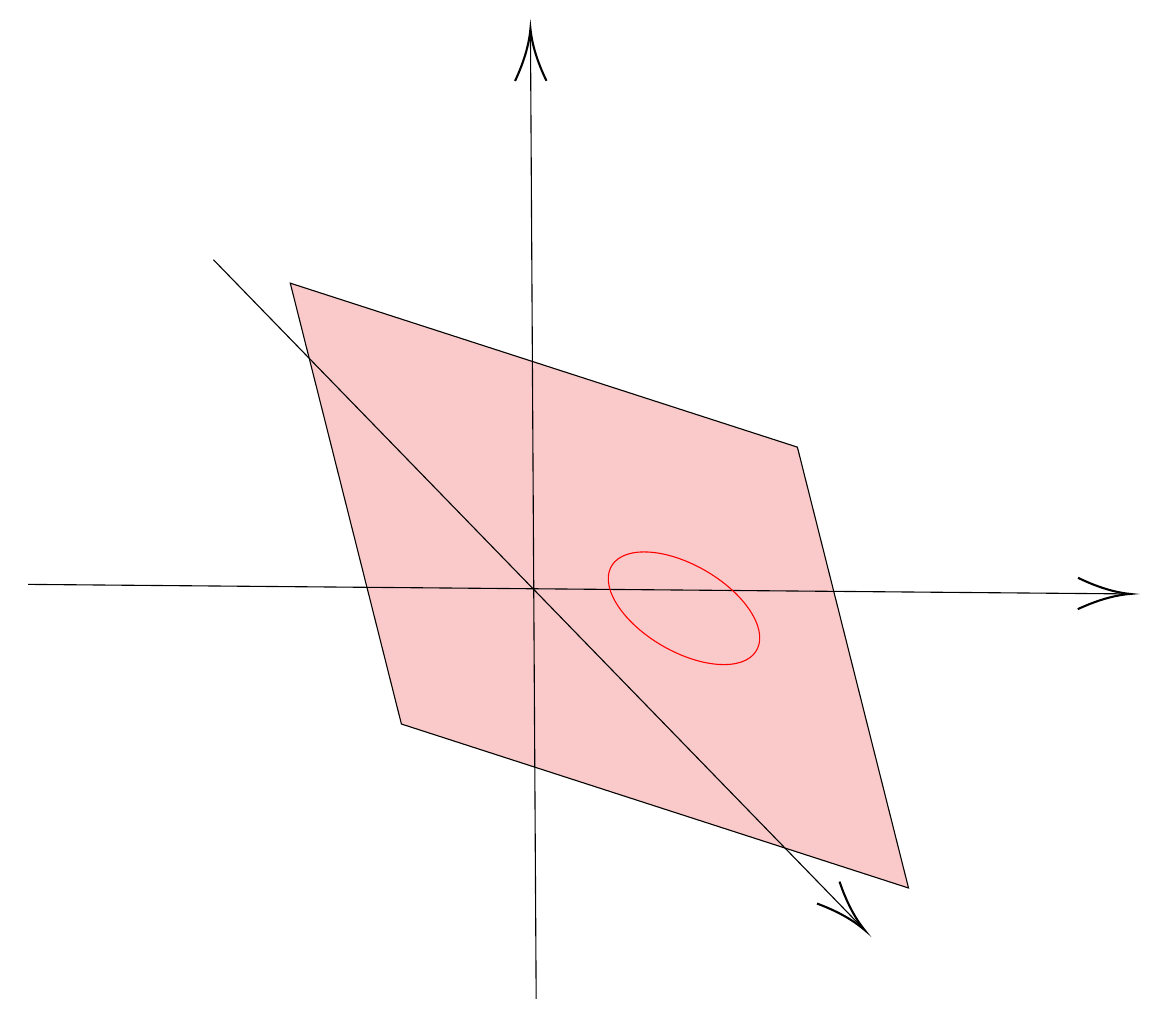
\begin{tikzpicture}[x=0.75pt,y=0.75pt,yscale=-2.3,xscale=2.3]
			%uncomment if require: \path (0,300); %set diagram left start at 0, and has height of 300

			%Shape: Parallelogram [id:dp3386268494356779] 
			\draw  [color={rgb, 255:red, 3; green, 0; blue, 0 }  ,draw opacity=1 ][fill={rgb, 255:red, 233; green, 27; blue, 27 }  ,fill opacity=0.23 ] (222.17,175.25) -- (198.89,82.9) -- (305.12,117.25) -- (328.4,209.6) -- cycle ;
			%Straight Lines [id:da5976315612243159] 
			\draw    (182.8,78) -- (317.81,216.97) ;
			\draw [shift={(319.2,218.4)}, rotate = 225.83] [color={rgb, 255:red, 0; green, 0; blue, 0 }  ][line width=0.75]    (10.93,-3.29) .. controls (6.95,-1.4) and (3.31,-0.3) .. (0,0) .. controls (3.31,0.3) and (6.95,1.4) .. (10.93,3.29)   ;
			%Straight Lines [id:da8891236273278385] 
			\draw    (250.4,232.8) -- (249.21,31.6) ;
			\draw [shift={(249.2,29.6)}, rotate = 89.66] [color={rgb, 255:red, 0; green, 0; blue, 0 }  ][line width=0.75]    (10.93,-3.29) .. controls (6.95,-1.4) and (3.31,-0.3) .. (0,0) .. controls (3.31,0.3) and (6.95,1.4) .. (10.93,3.29)   ;
			%Straight Lines [id:da4262954076409089] 
			\draw    (144,146) -- (372.8,147.98) ;
			\draw [shift={(374.8,148)}, rotate = 180.5] [color={rgb, 255:red, 0; green, 0; blue, 0 }  ][line width=0.75]    (10.93,-3.29) .. controls (6.95,-1.4) and (3.31,-0.3) .. (0,0) .. controls (3.31,0.3) and (6.95,1.4) .. (10.93,3.29)   ;
			%Shape: Ellipse [id:dp8850500969361768] 
			\draw  [color={rgb, 255:red, 255; green, 0; blue, 0 }  ,draw opacity=1 ] (267.87,151) .. controls (263.27,144.48) and (265.57,139.2) .. (273.03,139.2) .. controls (280.48,139.2) and (290.25,144.48) .. (294.86,151) .. controls (299.47,157.52) and (297.16,162.8) .. (289.71,162.8) .. controls (282.25,162.8) and (272.48,157.52) .. (267.87,151) -- cycle ;

			\end{tikzpicture}

			A parallel orthogal unit vector to this plane is $\langle 0, \frac{1}{\sqrt{2}}, -\frac{1}{\sqrt{2}} \rangle$. Finding the cross product and normalizing, we get $\langle -\frac{2}{\sqrt{6}}, \frac{1}{\sqrt{6}}, \frac{1}{\sqrt{6}} \rangle$ We can treat this as a basis for 2D coordinates on the given plane. Multiplying $2\sin(t)$ by the first and $2\cos(t)$ by the second respectively will give the parameterized terms. Then the total parametric equation of the circle is 
			\[ \boxed{\langle 1 - \frac{4}{\sqrt{6}}\cos(t), 2 + \sqrt{2}\sin(t) + \frac{2}{\sqrt{6}}\cos(t), 0 - \sqrt{2}\sin(t) + \frac{2}{\sqrt{6}}\cos(t) \rangle} \tag*{\qed} \]
			
		\end{solution}
		\clearpage
		\thequestion \part Find parametric equations for two circles $C_1$ and $C_2$ in space such that \begin{itemize}
			\item $C_1$ and $C_2$ have the same radius
			\item $C_1$ and $C_2$ intersect at the points (0, 1, 0) and (0, 0, 1) and nowhere else.
		\end{itemize}
			\begin{solution}
				We can create circles centered at (0, 0, 0) and (0, 1, 1) with radius 1. The equations for these would be 
				\begin{center}
					\[ \boxed {C_1 = \langle 0, \sin(t), \cos(t)} \] \\
					and
					\[\boxed{C_2 = \langle 0, 1 + \sin(t), 1 + \cos(t)} \tag*{\qed} \]
				\end{center}
			\end{solution}
	\end{parts}
\clearpage
%4 
\question Consider the curves C1 and C2 with parametrizations given by TODO
\clearpage
%5
\question The plane curve with parametrization $r(t) = \langle e^t \cos 2t, e^t \sin 2t\rangle, t \in \mathbb{R}$, is an example of a Bernoulli
spiral. Show that the angle $\varphi$ between the position vector $\mathbf{r}(t)$ and the tangent vector $\mathbf{r}'(t)$ is constant, and find the value of $\varphi$ in radians to two decimal places.
	\begin{solution}
		We find the dot product of the position and tangent vector:
		\begin{align*}
			\mathbf{r} \cdot \mathbf{r'} &= \langle e^t \cos 2t, e^t \sin 2t \rangle \cdot \langle e^t \cos 2t - 2e^t \sin 2t, e^t \sin 2t + 2e^t \cos 2t \rangle \\
			&= e^{2t} \cos^2 2t - e^{2t} \cos 2t \sin 2t + e^{2t} \sin^2 2t + e^{2t} \cos 2t \sin 2t \\
			& = e^{2t} \cos^2 2t + e^{2t} \sin^2 2t \\
			&= e^{2t}
		\end{align*}
		The norms of $\mathbf{r}$ and $\mathbf{r'}$ respectively are $e^t$ and $\sqrt{5}e^t$, so the cos of the angle is thus a constant $\frac{1}{\sqrt{5}}$. Then 
		\[ \arccos (\frac{1}{\sqrt{5}}) = \boxed{\varphi = 1.107148718} \tag*{\qed} \]
	\end{solution}
%6
\question A wheel of radius R traces out a cycloid.
	\begin{parts}
		\part Find a parametrization, $\mathbf{c} (t)$, of this cycloid such that a single arch is traced out from $t = 0$ to $t = 2\pi$ (a single revolution of the wheel). Choose your coordinate system so that $\mathbf{c} (0)= (0, 0)$.
		\begin{solution}
			\[ \boxed{\mathbf{c} (t) = \langle R(t-\sin(t)),\ R(1-\cos(t)) \rangle} \tag*{\qed}\]
		\end{solution}
		\part Find the length of a single arch.
			\begin{solution}
				\begin{align*}
					\int_{0}^{2\pi}\sqrt{\frac{dx}{dt}^2+\frac{dy}{dt}^2}dt &= \int_{0}^{2\pi}R\sqrt{(1-\cos(t))^2+(\sin(t))^2}dt \\
					&= \int_{0}^{2\pi}R\sqrt{2 - 2\cos(t)}dt \\
					&= \boxed{8R} \tag*{\qed}
				\end{align*}
			\end{solution}
	\end{parts}
\clearpage
%7
\question An \textit{involute} is the curve traced out by the end of a taut string being unwound from a given curve, in the plane of the curve. Let's consider the circle involute that arises when we unwind string from a spool. In the figure below the unwound string is shown in purple, the angle between the green line segment and the purple line segment is $\frac{\pi}{2}$, and the spool, which has radius R, is shown in orange. The circle involute is shown in black, and we wish to parametrize the circle involute in terms of the angle $\theta$; that is, we want to find a vector valued function $\mathbf{r}(\theta)$ for $\theta \geq 0$ so that its associated space curve is the circle involute.\\
\begin{center}
	\includegraphics*[scale=0.3]{images/03-involute.png}
\end{center}
	\begin{parts} 
		\part What is the length of the unwound thread (that is, the purple line segment) as a function of $\theta$?
			\begin{solution}
				Since the thread is taut around the circumference of the circle, it the length unraveled is equal to the arclength which $\theta$ has already passed through. This is equal to $\boxed{R\theta }$.
			\end{solution}
		\part What is $\mathbf{r}(\theta)$? Hint: It may help to first find the vector that moves from the origin to the edge ofthe circle (the green line in the diagram) and then find the vector that moves from the edge of the circle to the involute (the purple line in the diagram).
			\begin{solution}
				The green vector can simply use the parametric equation of a circle with radius $R$:  $\langle R\cos(\theta), R\sin(\theta) \rangle$. \\
				The purple vector is a vector with direction perpendicular to the radius and a magnitude equal to the length of the string. The direction can be given by $\langle \sin(\theta), -\cos(\theta) \rangle$. Multiplying by the magnitude, we get $\langle R\theta\sin(\theta), -R\theta\cos(\theta) \rangle$. Adding the two together, we find $\boxed{\mathbf{r}(\theta) = \langle R\cos(\theta) + R\theta\sin (\theta), R\sin(\theta) - R\theta\cos(\theta) \rangle}$. \qed
			\end{solution}
		\part What is the length of the curve from $\theta = 0$ to $\theta = b$?
			\begin{solution}
				Using the arclength formula:
				
				\begin{align*}
					\int_{0}^{b} \sqrt{(\frac{dx}{d\theta})^2+ (\frac{dx}{d\theta})^2} &= \int_{0}^{b} R\sqrt{(\theta \cos(\theta) + \sin(\theta) - \sin(\theta))^2 + (\theta \sin(\theta) + \cos(\theta) - \cos(\theta))^2} d\theta \\
					&= \int_{0}^{b} R\sqrt{(\theta \cos(\theta) )^2 + (\theta \sin(\theta))^2} d\theta \\
					&= \int_{0}^{b} R\sqrt{\theta^2} d\theta \\
					&= \int_{0}^{b} R\theta d\theta \\
					&= \boxed{\frac{Rb^2}{2}} \tag*{\qed}
				\end{align*}
			\end{solution}
		\part Parametrize the circle involute in terms of arc length.
			\begin{solution}
				We found the arclength $s=\frac{R\theta^2}{2}$. The parametrization in terms of $s$ is thus
				\[ \boxed{\mathbf{r}(s) = \langle R\cos\left(\sqrt{\frac{2s}{R}}\right) + R\sqrt{\frac{2s}{R}}\sin \left(\sqrt{\frac{2s}{R}}\right), R\sin\left(\sqrt{\frac{2s}{R}}\right) - R\sqrt{\frac{2s}{R}}\cos\left(\sqrt{\frac{2s}{R}}\right) \rangle} \]
			\end{solution}
		\part Compute the curvature of the circle involute. \textit{Hint:} The book contains several different ways to compute the curvature $\kappa$. Some may be easier than others. 
			\begin{solution}
				We can compute the curvature by calculating the magnitude of the derivative of the unit tangent vector $\bm{T'}(\theta)$ and dividing by the magnitude of the tangent vector $\mathbf{r'}(\theta)$. 
				The tangent vector is 
				\begin{align*}
					\mathbf{r'}(\theta) &= \langle -R\sin(\theta) + R\sin (\theta) + R\theta\cos(\theta), R\cos(\theta) - R\cos(\theta) + R\theta\sin(\theta)\rangle \\
					&= \langle R\theta\cos(\theta), R\theta\sin(\theta) \rangle
				\end{align*}
				Of course, the unit tangent vector is then just the parametric equation of a circle. The derivative of the unit tangent vector is still a parametric circle, so it has magnitude 1. The tangent vector has magnitude $R\theta$, so the curvature of the involute is \[\boxed{\frac{1}{R\theta}} \tag*{\qed}\]
			\end{solution}
	\end{parts}
\end{questions}

\end{document}